\documentclass[twoside,11pt]{article}
\usepackage[preprint]{jmlr2e}
\usepackage[utf8]{inputenc}
\usepackage[T1]{fontenc}
\usepackage{booktabs}
\usepackage{microtype}
\usepackage{amsmath}
\usepackage{xcolor}
\usepackage{url}
\hypersetup{colorlinks=true,citecolor=blue,linkcolor=blue,urlcolor=blue}
\graphicspath{{figures/}}
\emergencystretch=2em

% Keep true for double-blind submission; switch to \anonymousfalse only for camera-ready.
\newif\ifanonymous
\anonymoustrue

\title{TabAL: Molecular Representation Changes Active-Learning Performance and Model Rankings}
\ifanonymous
\author{\name Anonymous Authors}
\ShortHeadings{Representation Changes Molecular Active Learning}{Anonymous Authors}
\else
\author{\name Satya Pratik Srivastava \email ss864@snu.edu.in \\
\addr Shiv Nadar University, Delhi-NCR, India
\AND
\name Vaidehi Saxena \email vs529@snu.edu.in \\
\addr Shiv Nadar University, Delhi-NCR, India
\AND
\name Harshit Singh \email hs494@snu.edu.in \\
\addr Shiv Nadar University, Delhi-NCR, India
\AND
\name Rajeev Kumar Singh \email rajeev.kumar@snu.edu.in \\
\addr Shiv Nadar University, Delhi-NCR, India}
\ShortHeadings{Representation Changes Molecular Active Learning}{Srivastava, Saxena, Singh, and Singh}
\fi
\firstpageno{1}

\begin{document}
\maketitle

\begin{abstract}
Molecular representation is often fixed before an active-learning benchmark, although it can determine how effectively a learner uses a small labeled set. We quantify this dependence by comparing 1,024-bit ECFP4 fingerprints with 210 standardized RDKit2D descriptors for TabPFN v2.5, random forest, XGBoost, and LightGBM on five scaffold-split ADMET classification tasks. The fully paired benchmark contains three acquisition policies, ten acquisition seeds, fifteen label budgets from 32 to 256, and 1,200 trajectories. Averaged over matched datasets and seeds, RDKit2D increases normalized AUROC area under the learning curve (AULC) by 0.070 (95\% paired-bootstrap confidence interval 0.066--0.074). All twelve model--policy macro averages improve by 0.054--0.091, but this pattern is not universal at the endpoint level: random forest decreases by 0.011 on P-glycoprotein. Representation also changes the comparative conclusion. Under ECFP4, the strongest macro condition is random forest with entropy--diversity acquisition (0.796); under RDKit2D, TabPFN with entropy--diversity has the largest point estimate (0.857) but is statistically tied with random forest (0.855). Complete AUPRC, Brier, negative log-likelihood, query-similarity, and runtime results show that the trade-offs extend beyond AUROC. These results establish representation as an experimental factor in active-learning comparisons rather than a neutral preprocessing choice.
\end{abstract}

\begin{keywords}
molecular active learning, molecular representation, TabPFN, ADMET, scaffold split, label efficiency
\end{keywords}

\section{Introduction}
Active learning (AL) seeks to reduce experimental labeling by repeatedly selecting informative examples from an unlabeled pool \citep{settles2009active}. This premise is attractive in molecular discovery, where wet-lab labels may be slow or expensive to obtain and the available chemical library can be much larger than the assay budget \citep{graff2021molpal}. An AL result, however, is produced by a coupled system: a molecular representation, predictive model, acquisition rule, initialization, and evaluation protocol. Changing one component may change not only predictive accuracy but also the molecules queried in every subsequent round.

Molecular representations encode different inductive assumptions. ECFP fingerprints describe local circular substructures as sparse binary indicators \citep{rogers2010ecfp}, whereas RDKit2D provides dense numerical descriptors of physicochemical and topological properties \citep{landrum2024rdkit}. Representation effects are well established in static molecular prediction \citep{yang2019analyzing}, and recent work has begun to examine them in molecular AL directly. Controlled benchmarking under scaffold split found that acquisition rankings depend on whether models use ECFP or ChemBERTa representations \citep{wu2026controlled}. ActiveFusion compared fingerprints, descriptors, graph representations, Transformer embeddings, and feature fusion on regression tasks, showing substantial representation--acquisition interactions \citep{evbarunegbe2026activefusion}. In parallel, Tab-AICL formulated active in-context learning for TabPFN on general tabular classification benchmarks \citep{treerath2026active}. Therefore, the open question is not whether representation can matter in AL, but how a compact descriptor--fingerprint comparison changes conclusions about a tabular foundation model relative to strong classical baselines in low-label ADMET classification.

TabPFN is a relevant stress test for this question. It is pretrained on synthetic numerical tables and has demonstrated strong small-data performance \citep{hollmann2025accurate}, including promising molecular applications \citep{chen2026tabpfn,benhicham2026molecular}. Its inductive bias differs from that of tree ensembles, and sparse 1,024-bit fingerprints differ markedly from the dense tables used in pretraining. A benchmark that fixes ECFP4 could consequently measure compatibility with one representation as much as general low-label ability.

We make three contributions. First, we use a fully paired design to isolate representation effects across four learners, three acquisition policies, five endpoints, and ten acquisition seeds. Second, we report label efficiency, ranking quality, probability quality, chemical redundancy, and runtime rather than relying on a single endpoint metric. Third, we distinguish macro conclusions from endpoint-level exceptions and quantify uncertainty using paired bootstrap intervals. The evidence supports a bounded conclusion: the selected representation can alter both AL performance and model ranking, but neither RDKit2D nor TabPFN is universally best.

\begin{figure}[!htbp]
  \centering
  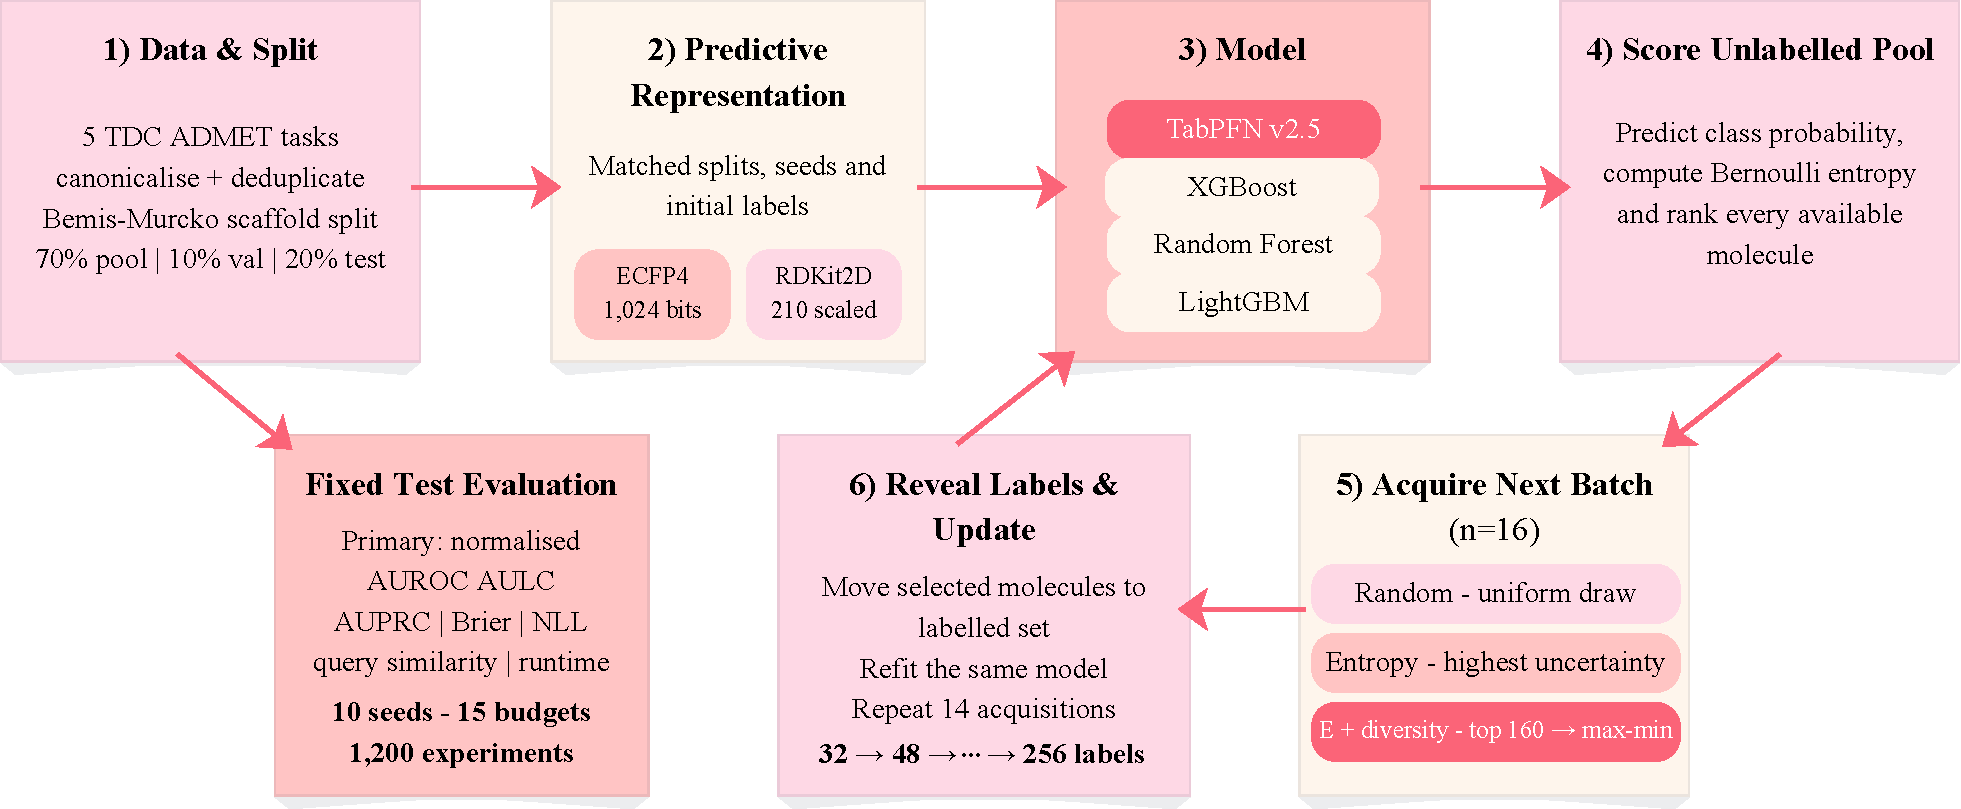
\includegraphics[width=\textwidth]{fig1.pdf}
  \caption{\textbf{Paired molecular active-learning protocol.} Five TDC ADMET tasks are canonicalized, deduplicated, and divided by a fixed Bemis--Murcko scaffold split. Matched ECFP4 and RDKit2D representations are evaluated with four learners. Starting from 32 labeled molecules, the system acquires batches of 16 by random, entropy, or entropy--diversity selection, refits the learner, and evaluates on an untouched test set through a budget of 256 labels.}
  \label{fig:pipeline}
\end{figure}

\section{Related Work}
\paragraph{Molecular active learning.}
Pool-based molecular AL has been studied for virtual screening, property prediction, and structural exploration. MolPAL demonstrated that learned surrogate models and uncertainty-aware acquisition can accelerate virtual screening \citep{graff2021molpal}. Diversity-aware batch selection addresses redundancy among simultaneously acquired examples, a general concern in batch AL \citep{sener2018coreset,biyik2019dpp}. These studies motivate our random, entropy, and entropy--diversity policies, but our objective is comparative: we ask whether a model ranking survives a representation change under otherwise matched conditions.

\paragraph{Representation effects in AL.}
Our work is closest to Controlled Benchmarking and ActiveFusion. Controlled Benchmarking evaluates five acquisition strategies on seven ADME tasks using ECFP-MLP and ChemBERTa-MLP models; it emphasizes acquisition performance across representation slices \citep{wu2026controlled}. ActiveFusion spans descriptors, fingerprints, GNNs, Transformers, and fused representations on four regression tasks and emphasizes representation fusion and chemical-space exploration \citep{evbarunegbe2026activefusion}. Our study is complementary rather than the first treatment of representation in molecular AL: it focuses on binary ADMET classification, a dense descriptor versus sparse fingerprint contrast, and a paired comparison of TabPFN with three tree ensembles. The central estimand is the representation-induced change in model and policy comparisons.

\paragraph{Tabular foundation models.}
TabPFN performs in-context prediction using priors learned from synthetic tabular tasks \citep{hollmann2025accurate}. Molecular studies indicate that descriptor choice can strongly affect static TabPFN performance \citep{chen2026tabpfn,benhicham2026molecular}. Tab-AICL recently extended foundation models to an iterative context-selection setting on 20 general classification datasets and compared uncertainty, diversity, and hybrid acquisition \citep{treerath2026active}. We instead hold the AL protocol fixed and examine whether a molecular representation changes TabPFN's relative position against random forest, XGBoost, and LightGBM. The three classical models were chosen as widely used, computationally mature tabular baselines with distinct bagging and boosting behavior. They do not span all model families; neural graph models and Gaussian processes remain important omissions.

\section{Experimental Design}
\subsection{Datasets, cleaning, and scaffold splits}
We use five binary endpoints from Therapeutics Data Commons (TDC) \citep{huang2021tdc}: drug-induced liver injury (DILI), human intestinal absorption (HIA Hou), oral bioavailability (Bioavailability Ma), P-glycoprotein inhibition (Pgp Broccatelli), and blood--brain barrier penetration (BBB Martins). SMILES are canonicalized with RDKit. Invalid records are removed, identical duplicate records are collapsed, and duplicate structures with conflicting labels are excluded. Table~\ref{tab:data} reports the resulting task sizes and prevalences.

We construct one deterministic 70/10/20 Bemis--Murcko scaffold partition per endpoint using seed 42 \citep{bemis1996frameworks}. The 70\% training partition serves as the AL pool and the 20\% test partition remains untouched throughout acquisition. The 10\% validation partition is retained but not used: all hyperparameters are fixed before comparison. This design avoids representation-specific tuning, but it does not establish that each model is equally close to its optimum in both feature spaces. We return to this trade-off in Section~\ref{sec:limitations}.

\begin{table}[t]
\centering
\small
\caption{Dataset characteristics after canonicalization and deduplication. Pool and test sizes correspond to the fixed scaffold partition used in all paired runs.}
\label{tab:data}
\begin{tabular}{lrrrrr}
\toprule
Endpoint & $N$ & Positive rate & Pool $N$ & Test $N$ & Scaffolds \\
\midrule
DILI & 475 & 0.497 & 379 & 96 & 311 \\
HIA Hou & 578 & 0.865 & 461 & 117 & 385 \\
Bioavailability Ma & 640 & 0.769 & 512 & 128 & 440 \\
Pgp Broccatelli & 1,212 & 0.534 & 969 & 243 & 682 \\
BBB Martins & 1,965 & 0.763 & 1,571 & 394 & 1,020 \\
\bottomrule
\end{tabular}
\end{table}

\subsection{Representations}
ECFP4 uses radius 2, 1,024 bits, no chirality, and no feature invariants \citep{rogers2010ecfp}. RDKit2D begins with 210 scalar descriptors from RDKit 2023.09.6 \citep{landrum2024rdkit}. Non-finite descriptor values are replaced using statistics computed only from the current labeled training set, after which each descriptor is standardized using the labeled-set mean and standard deviation. The transformation is refit at each round and applied to the unlabeled pool and fixed test set; test or validation data are never used to estimate preprocessing parameters. Chemical diversity is evaluated with ECFP4 Tanimoto similarity for both predictive representations so that the diversity scale remains common.

\subsection{Models and fixed configurations}
We compare TabPFN v2.5 with eight estimators, random forest with 500 trees, XGBoost with 300 depth-4 trees, and LightGBM with 300 trees and 31 leaves \citep{breiman2001random,chen2016xgboost,ke2017lightgbm}. Appendix~\ref{app:hyper} lists the complete configurations. Hyperparameters are identical across datasets and representations and were not selected using the held-out validation split. This deliberate fixed-configuration design isolates the effect of changing the representation for a given implementation, but it should not be interpreted as a tuned leaderboard.

The baseline set covers a pretrained tabular foundation model, bagged decision trees, and two gradient-boosting implementations. Random forest, XGBoost, and LightGBM are strong baselines for small tabular datasets and accommodate both sparse binary and dense continuous inputs. However, all three are tree ensembles. The experiment therefore does not determine whether the same interaction holds for kernel methods, Gaussian processes, multilayer perceptrons, graph neural networks, or more recent TabPFN generations such as TabPFN3.

\subsection{Acquisition protocol}
For each endpoint and seed, the initial 32 examples are drawn without replacement by consecutive calls to a seeded pseudo-random generator. The exact same initial molecule identities and tie-breaking order are reused across representations, models, and acquisition policies. Each round adds 16 examples until the labeled set reaches 256, producing fifteen evaluated budgets: $32,48,\ldots,256$.

Random acquisition draws uniformly from the remaining pool. Entropy acquisition ranks molecules by Bernoulli predictive entropy
\begin{equation}
H(p)=-p\log p-(1-p)\log(1-p).
\end{equation}
Entropy--diversity first retains the 160 highest-entropy candidates and then greedily selects a batch that maximizes the minimum ECFP4 Tanimoto distance to the labeled set and to molecules already selected in the batch. This two-stage rule tests whether structural dispersion adds value after uncertainty filtering.

\subsection{Metrics and statistical analysis}
At each budget $b_k$, the primary score is test AUROC $A_k$. Normalized AULC is the trapezoidal integral divided by the budget range,
\begin{equation}
\mathrm{AULC}=\frac{1}{b_K-b_1}\sum_{k=1}^{K-1}\frac{A_k+A_{k+1}}{2}(b_{k+1}-b_k),
\end{equation}
so its scale remains that of AUROC. Secondary metrics are AUPRC, Brier score, negative log-likelihood (NLL), mean within-batch ECFP4 Tanimoto similarity, and wall-clock runtime. ``Best condition per dataset'' means the model--policy pair with the highest AULC after averaging its ten seeds within that dataset and representation.

Representation comparisons are paired on endpoint, seed, learner, and acquisition policy. We report percentile intervals from 10,000 paired bootstrap resamples with seed 42. For a model--policy macro condition, the bootstrap unit is one of the 50 endpoint--seed trajectories. For endpoint summaries, the unit is one of 120 model--policy--seed pairs. These intervals quantify acquisition-seed and condition variability under the single fixed data split; they do not quantify split-to-split uncertainty. More than thirty pairwise contrasts were examined. Their intervals are exploratory and unadjusted for multiplicity, so marginal exclusions of zero are not interpreted as definitive significance.

\section{Results}
\subsection{Representation changes label efficiency and model ranking}
\begin{figure}[!htbp]
  \centering
  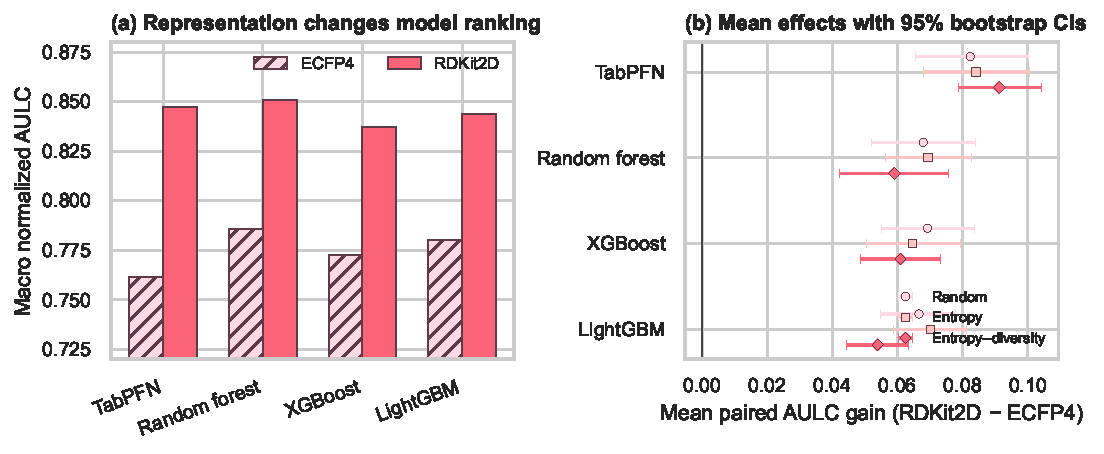
\includegraphics[width=\textwidth]{figure_main_ci.pdf}
  \caption{\textbf{Representation effects on label efficiency.} (a) Macro normalized AULC averaged over policies, datasets, and seeds. (b) Mean paired RDKit2D-minus-ECFP4 AULC effects for every model--policy condition; bars are 95\% paired-bootstrap confidence intervals over 50 matched endpoint--seed trajectories. Unlike the earlier boxplot, panel (b) depicts uncertainty in the mean effect relevant to the central claim.}
  \label{fig:main}
\end{figure}

Across all 600 matched trajectory pairs, RDKit2D increases normalized AULC by 0.070 (95\% CI 0.066--0.074). The mean effect is positive in every one of the twelve model--policy macro conditions (Figure~\ref{fig:main}b), ranging from 0.054 for LightGBM with entropy--diversity to 0.091 for TabPFN with entropy--diversity. This result does not mean that RDKit2D wins every endpoint-level comparison. The claim is specifically about model--policy averages over five tasks.

Under ECFP4, random forest with entropy--diversity has the highest macro AULC (0.796), closely followed by LightGBM with entropy--diversity (0.795); TabPFN with entropy--diversity reaches 0.766. Under RDKit2D, the largest point estimate is TabPFN with entropy--diversity (0.857), followed by random forest with entropy--diversity (0.855) and random forest with entropy (0.853). The paired TabPFN-minus-random-forest contrast at the best RDKit2D policy is only 0.0026 and its interval includes zero. We therefore describe these methods as statistically tied rather than claiming that TabPFN is unambiguously best.

The interaction remains substantial even under this conservative interpretation. Under entropy--diversity, the representation change improves the paired TabPFN-minus-random-forest contrast by 0.032 (95\% CI 0.022--0.043), the TabPFN-minus-XGBoost contrast by 0.030 (0.019--0.042), and the TabPFN-minus-LightGBM contrast by 0.037 (0.027--0.049). Under random acquisition, the corresponding interaction estimates are 0.014, 0.013, and 0.016. Thus, RDKit2D disproportionately benefits TabPFN relative to each tree ensemble, even though its best absolute score is tied with random forest.

\begin{figure}[!htbp]
  \centering
  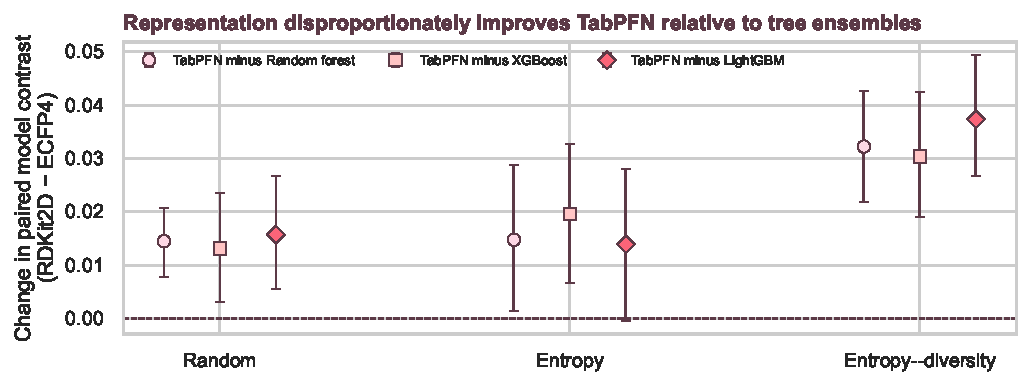
\includegraphics[width=.86\textwidth]{figure_interaction.pdf}
  \caption{\textbf{Representation-by-model interaction.} Change from ECFP4 to RDKit2D in the paired TabPFN-minus-tree AULC contrast. Positive values mean that RDKit2D benefits TabPFN more than the indicated comparator. Intervals use 50 matched endpoint--seed trajectories for each acquisition policy.}
  \label{fig:interaction}
\end{figure}

\subsection{Endpoint heterogeneity limits the macro conclusion}
\begin{figure}[!htbp]
  \centering
  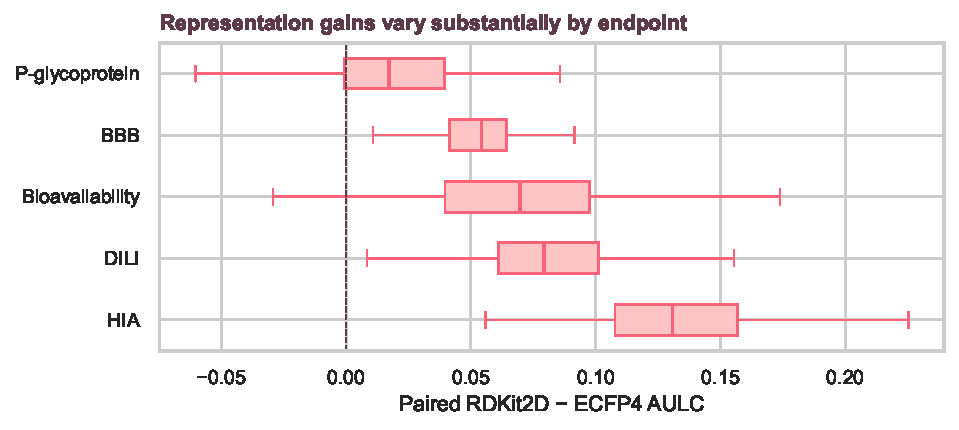
\includegraphics[width=.82\textwidth]{figure_endpoint_boxplots.pdf}
  \caption{\textbf{Endpoint heterogeneity in representation gains.} Each box summarizes 120 paired RDKit2D-minus-ECFP4 AULC differences (four learners, three policies, and ten seeds); whiskers extend to 1.5 IQR. This distributional view is retained from the original paper, while Figure~\ref{fig:main} provides confidence intervals for the mean macro effects.}
  \label{fig:endpoints}
\end{figure}

Mean representation gains vary from 0.132 on HIA to 0.016 on P-glycoprotein (Figure~\ref{fig:endpoints}). The intermediate gains are 0.081 for DILI, 0.067 for bioavailability, and 0.053 for BBB. Random forest on P-glycoprotein is the sole model-by-endpoint exception to the overall direction, decreasing by 0.011 on average across acquisition policies. This cell directly rules out the stronger statement that RDKit2D improves every setting.

The best model is likewise endpoint-dependent. Under RDKit2D, random forest provides the largest condition average on BBB, bioavailability, and DILI, whereas TabPFN provides the largest point estimate on HIA and P-glycoprotein. Endpoint size, prevalence, scaffold composition, and descriptor relevance may all contribute, but the present design cannot separate these explanations with only five datasets.

\subsection{Acquisition policy effects are smaller than representation effects}
Within RDKit2D, entropy--diversity improves over random acquisition by 0.0161 for TabPFN (95\% CI 0.0058--0.0274), 0.0096 for random forest (0.0029--0.0169), 0.0146 for XGBoost (0.0055--0.0235), and 0.0144 for LightGBM (0.0066--0.0223). Entropy alone improves random forest and LightGBM relative to random sampling, while the TabPFN and XGBoost intervals include zero. Entropy--diversity does not reliably exceed entropy after pairing. Accordingly, the evidence supports a consistent benefit over random acquisition, not a universal advantage over uncertainty alone.

The ordering of effect sizes is informative: changing from ECFP4 to RDKit2D produces macro gains of 0.054--0.091, whereas changing acquisition policy within RDKit2D yields gains over random sampling of roughly 0.010--0.016. In this benchmark, representation choice is at least as consequential as the policy refinement being evaluated.

\begin{figure}[!htbp]
  \centering
  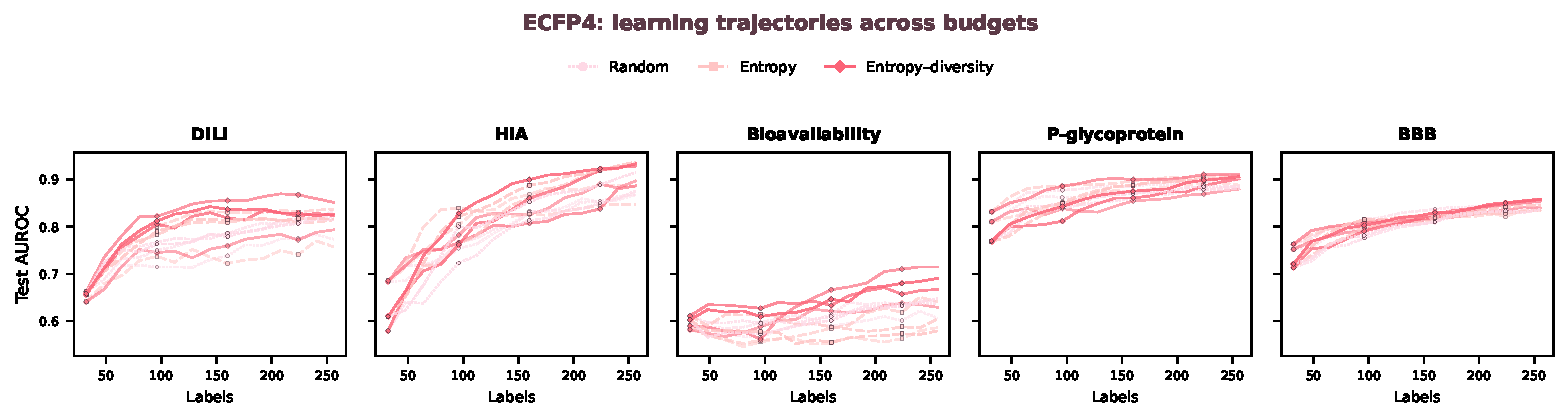
\includegraphics[width=.96\textwidth]{learning_curves_ecfp4_pink.pdf}
  \caption{\textbf{ECFP4 learning trajectories.} Test AUROC from 32 to 256 labeled molecules for every learner and acquisition policy. Line patterns and markers distinguish acquisition policies while the Figure~\ref{fig:pipeline} palette maintains visual consistency.}
  \label{fig:learning-ecfp4}
\end{figure}

\begin{figure}[!htbp]
  \centering
  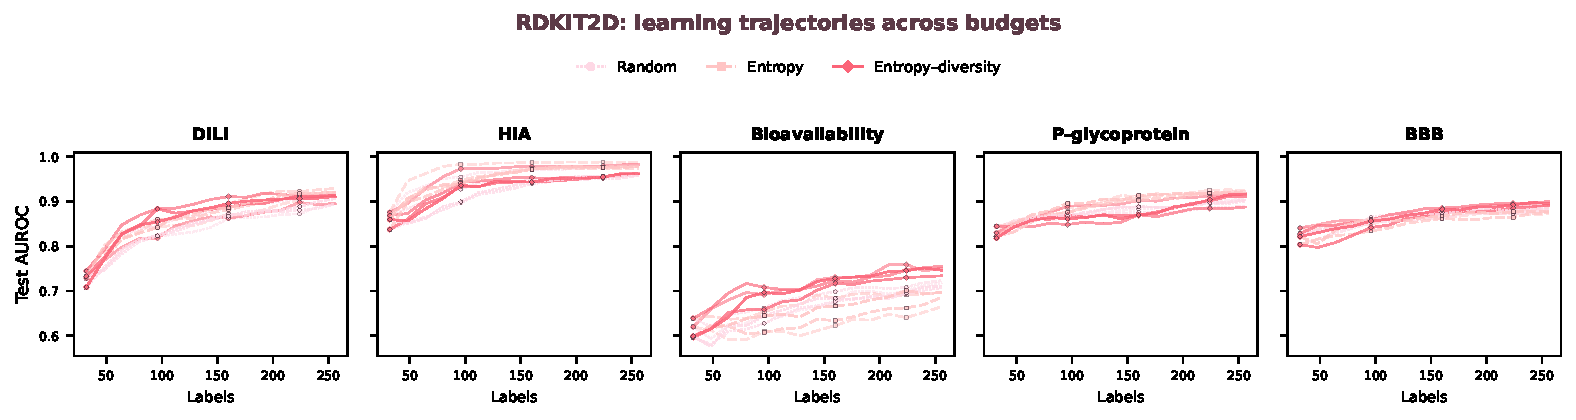
\includegraphics[width=.96\textwidth]{learning_curves_rdkit2d_pink.pdf}
  \caption{\textbf{RDKit2D learning trajectories.} Test AUROC over the same label budgets, learners, and acquisition policies as Figure~\ref{fig:learning-ecfp4}. The separated panel preserves legibility when placed within the results narrative.}
  \label{fig:learning-rdkit2d}
\end{figure}

\begin{figure}[!htbp]
  \centering
  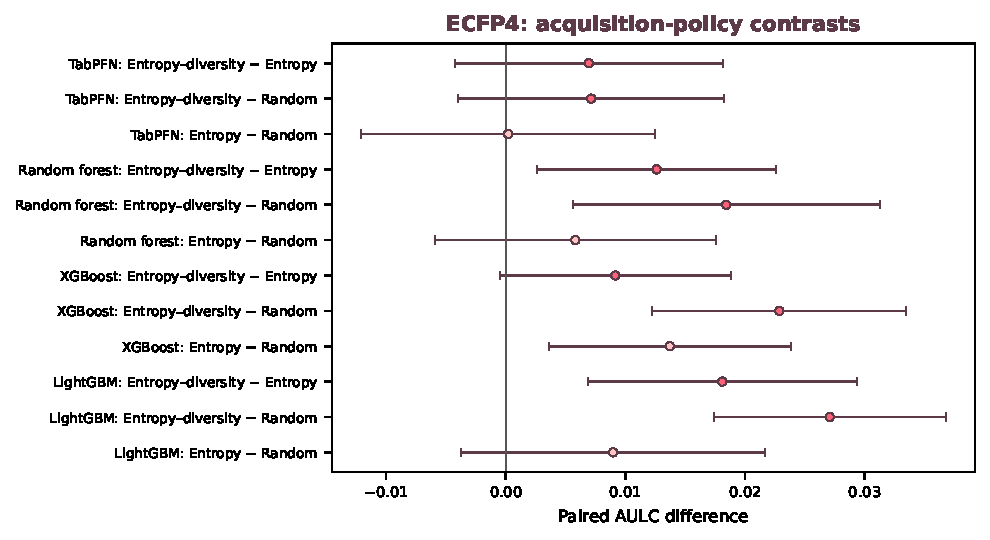
\includegraphics[width=.86\textwidth]{acquisition_ecfp4_pink.pdf}
  \caption{\textbf{Acquisition-policy contrasts with ECFP4.} Mean paired AULC differences and 95\% normal-approximation intervals across matched endpoint--seed trajectories.}
  \label{fig:acquisition-ecfp4}
\end{figure}

\begin{figure}[!htbp]
  \centering
  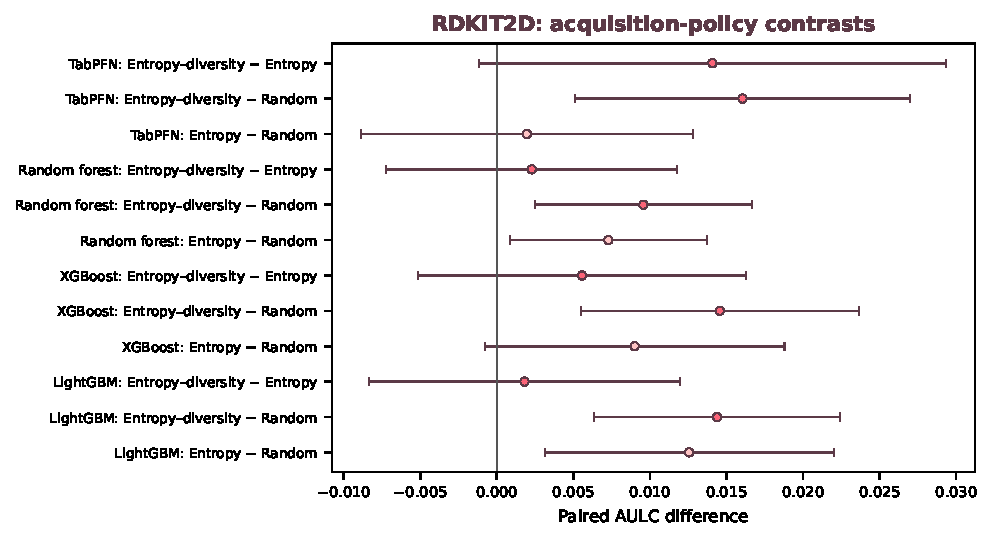
\includegraphics[width=.86\textwidth]{acquisition_rdkit2d_pink.pdf}
  \caption{\textbf{Acquisition-policy contrasts with RDKit2D.} The separated representation-specific panel keeps the policy comparison adjacent to the corresponding results while avoiding a dense full-page composite.}
  \label{fig:acquisition-rdkit2d}
\end{figure}

\subsection{Probability quality and runtime expose different trade-offs}
\begin{figure}[!htbp]
  \centering
  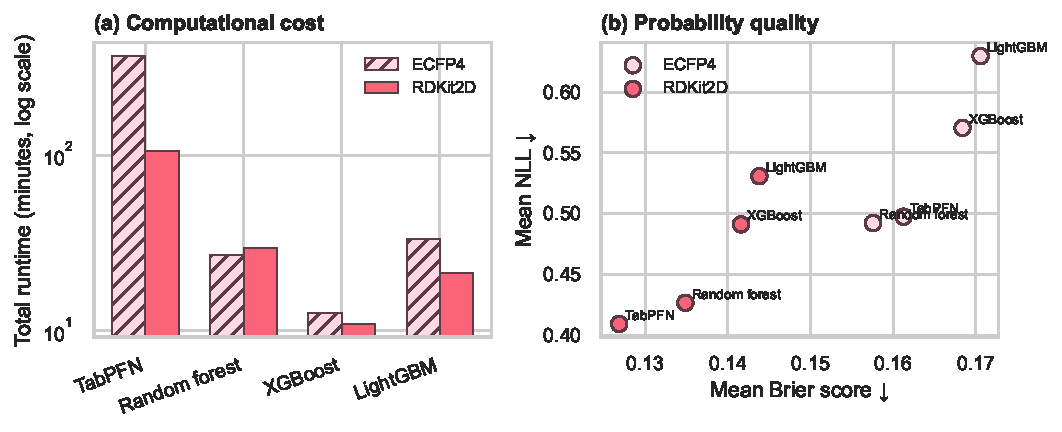
\includegraphics[width=\textwidth]{figure_secondary_metrics.pdf}
  \caption{\textbf{Secondary outcomes.} (a) Cumulative wall-clock time over all endpoints, seeds, budgets, and acquisition policies, shown on a logarithmic axis. (b) Mean Brier score and NLL averaged over datasets, seeds, budgets, and policies; lower is better for both. Labels identify learners.}
  \label{fig:secondary}
\end{figure}

The secondary results are summarized in Table~\ref{tab:secondary}. Random forest with RDKit2D and entropy--diversity obtains the largest mean AUPRC (0.916). TabPFN with RDKit2D and entropy provides the lowest Brier score (0.122) and NLL (0.395). These metrics answer different questions: AUPRC measures positive-class ranking under imbalance, whereas Brier score and NLL evaluate probability quality \citep{guo2017calibration}. Better test-set calibration does not automatically imply better ranking of unlabeled molecules for acquisition.

Runtime varies by more than an order of magnitude across learners. Averaged across policies, TabPFN takes 122.1 minutes per complete ECFP4 condition and 35.2 minutes per RDKit2D condition; the latter is a 71\% reduction. XGBoost is fastest at 4.2 and 3.7 minutes, respectively. The reduction for TabPFN is measured rather than inferred, but hardware contention and implementation details make runtime an engineering result rather than an architecture-independent property.

\begin{table}[t]
\centering
\small
\caption{Secondary metrics averaged over acquisition policies, datasets, seeds, and budgets. Runtime is the mean total minutes for one representation--model--policy condition over all five datasets and ten seeds. Arrows indicate preferred direction.}
\label{tab:secondary}
\begin{tabular}{llrrrr}
\toprule
Representation & Model & AUPRC $\uparrow$ & Brier $\downarrow$ & NLL $\downarrow$ & Runtime min $\downarrow$ \\
\midrule
ECFP4 & TabPFN & .860 & .161 & .497 & 122.1 \\
 & Random forest & .873 & .158 & .492 & 9.0 \\
 & XGBoost & .868 & .168 & .571 & 4.2 \\
 & LightGBM & .873 & .171 & .630 & 11.1 \\
\midrule
RDKit2D & TabPFN & .903 & \textbf{.127} & \textbf{.409} & 35.2 \\
 & Random forest & \textbf{.913} & .135 & .427 & 9.9 \\
 & XGBoost & .904 & .142 & .491 & \textbf{3.7} \\
 & LightGBM & .907 & .144 & .531 & 7.1 \\
\bottomrule
\end{tabular}
\end{table}

\subsection{Representation changes the selected molecules}
\begin{figure}[!htbp]
  \centering
  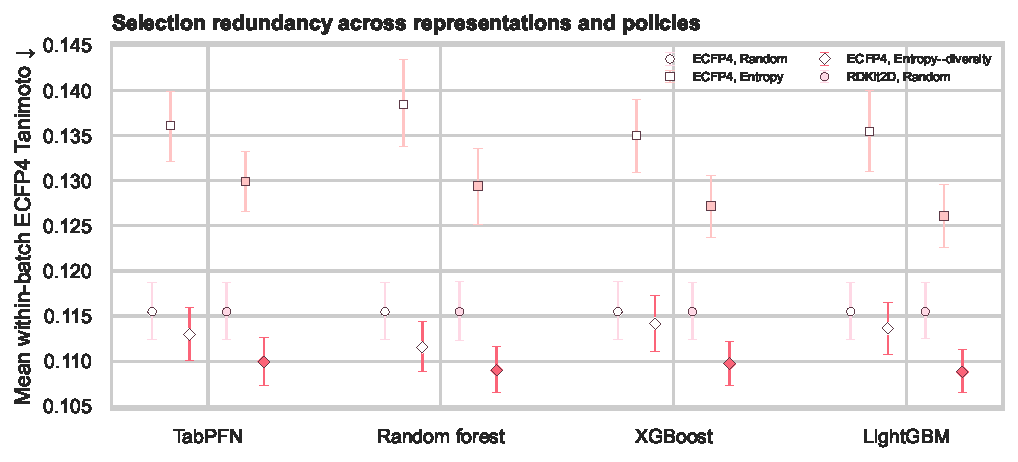
\includegraphics[width=.9\textwidth]{figure_diversity.pdf}
  \caption{\textbf{Selected-molecule redundancy.} Mean within-batch ECFP4 Tanimoto similarity across endpoints and acquisition seeds, with 95\% bootstrap intervals. Filled markers denote RDKit2D and open markers ECFP4. Lower similarity indicates more structurally diverse batches.}
  \label{fig:diversity}
\end{figure}

Entropy--diversity produces lower within-batch similarity than entropy acquisition for every learner and representation (Figure~\ref{fig:diversity}). Random acquisition is identical across learners and representations by construction because paired runs reuse the same seeded draw order. With entropy alone, RDKit2D produces mean similarities of 0.126--0.130, compared with 0.135--0.139 under ECFP4. Since similarity is always measured in the common ECFP4 space, this difference reflects a change in the molecules ranked as uncertain rather than a change in the metric itself.

The result is consistent across the aggregate but should not be conflated with a direct causal explanation for the AULC gain. RDKit2D changes fitted probabilities, the uncertainty ordering, and consequently the future labeled set. The present analysis shows that query paths diverge; it does not identify which queried substructures are responsible for improved prediction.

\section{Discussion}
\subsection{What the ranking reversal does and does not establish}
The most robust result is not that one learner wins. It is that the answer to ``which learner is strongest?'' changes when the molecular features change. Under ECFP4, the strongest macro conditions are tree ensembles. Under RDKit2D, TabPFN's point estimate rises to the top but remains tied with random forest. Reporting only the ECFP4 benchmark would make TabPFN appear uniformly weak; reporting only the RDKit2D benchmark could invite an unsupported claim of universal foundation-model superiority. The paired comparison exposes both narratives as representation-conditional.

One plausible mechanism is alignment between dense continuous descriptors and TabPFN's pretraining distribution. ECFP4 is sparse, high-dimensional, binary, and dominated by local substructure indicators, whereas RDKit2D is lower-dimensional, dense, and continuous. However, the comparison changes dimensionality, sparsity, scaling, and chemical information simultaneously. It cannot identify which characteristic produces the interaction. Controlled transformations---bit-density matching, descriptor binarization, dimensionality reduction, and additional fingerprint radii---would be needed to test this explanation.

The small TabPFN--random-forest difference under the best RDKit2D condition is also important. A point estimate separated by thousandths is not a stable basis for proclaiming a winner. The paired interval includes zero, and our many exploratory contrasts are unadjusted. The defensible conclusion is that TabPFN becomes competitive with random forest and improves more from the representation change, not that it dominates every conventional model.

\subsection{Implications for active-learning benchmarks}
AL benchmarks often standardize splits, seeds, and budgets but treat representation as fixed infrastructure. Our results suggest that representation should instead be crossed with the model, particularly when comparing learners with different inductive biases. At minimum, benchmark reports should include one fingerprint and one descriptor representation, preserve matched initial labeled sets, and report paired contrasts. If resources permit, learned graph and pretrained chemical language representations should be added.

Secondary outcomes should also be visible. A configuration with slightly lower AULC may be preferable if it is substantially faster, better calibrated, or selects more diverse chemistry. Here, XGBoost is much faster than TabPFN but does not lead the AULC table; random forest gives the strongest AUPRC; TabPFN gives the best mean probability scores under RDKit2D; and entropy--diversity reduces query redundancy without consistently beating entropy in AULC. No single scalar captures these trade-offs.

The fixed-hyperparameter protocol has a specific interpretation. Because neither representation is tuned, it avoids granting one side additional optimization effort and measures a reproducible out-of-the-box comparison. Conversely, the same setting can be differently appropriate for 1,024 sparse bits and 210 dense descriptors. A future nested design should tune each model--representation cell only on the validation split, then compare whether the interaction survives. The current unused validation partition is reserved for precisely that confirmation experiment.

\subsection{Limitations}\label{sec:limitations}
Every endpoint uses one scaffold split, so the ten seeds quantify variation in initialization and acquisition rather than train--test chemical geometry; multiple scaffold or simulated temporal splits are needed before generalizing the effect sizes. The benchmark also contains only five public binary ADMET tasks, two handcrafted representations, three tree ensembles, and TabPFN v2.5 rather than newer TabPFN generations, leaving regression, learned representations, kernel methods, neural and graph models, and broader chemical domains untested. Fixed hyperparameters preserve a controlled comparison but may favor one representation, and the exploratory confidence intervals are unadjusted for multiplicity. Finally, retrospective label revelation omits assay failure, batch effects, synthesis constraints, and distribution shifts encountered in prospective campaigns.

\section{Conclusion}
Molecular representation is an active component of the learning system. In this paired benchmark, replacing ECFP4 with RDKit2D increases macro AULC in all twelve model--policy combinations and benefits TabPFN disproportionately, yet one endpoint--model cell reverses direction and the best RDKit2D TabPFN condition is statistically tied with random forest. Representation also changes query redundancy, probability quality, and runtime. The practical lesson is methodological: comparative claims in molecular active learning should be conditioned on representation, supported with paired uncertainty, and checked across endpoints rather than inferred from a single preprocessing choice.

\appendix
\section{Model and protocol details}\label{app:hyper}
\begin{table}[h]
\centering
\small
\caption{Fixed model configurations used in every endpoint and representation.}
\begin{tabular}{p{.18\textwidth}p{.73\textwidth}}
\toprule
Model & Configuration \\
\midrule
TabPFN v2.5 & 8 estimators; probability balancing disabled; official v2.5 classifier checkpoint; device selected automatically. \\
Random forest & 500 trees; unlimited depth; $\sqrt{d}$ candidate features per split; minimum leaf size 1; bootstrap enabled; no class weighting; all CPU cores. \\
XGBoost & 300 trees; learning rate .05; depth 4; minimum child weight 1; row and column subsampling .8; no $\ell_1$ penalty; $\ell_2=1$; histogram tree method. \\
LightGBM & 300 trees; learning rate .05; 31 leaves; unlimited depth; minimum child samples 5; row and column subsampling .8; deterministic column-wise training. \\
\bottomrule
\end{tabular}
\end{table}

The active-learning seeds are 0--9. Initial sets use consecutive generator draws without replacement. Ties use a fixed seeded random order. Random acquisition reuses that order, explaining why its query-similarity observations are identical across models and representations. All predictive metrics are computed on the same untouched test indices at all fifteen budgets. Runtime is excluded from deterministic validation because operating-system scheduling and accelerator contention are not reproducible bit-for-bit.

\subsection{Interpretation of uncertainty}
Box-and-whisker plots describe the distribution of trajectory-level effects; they do not directly show uncertainty in the mean effect. Figure~\ref{fig:endpoints} is therefore used only to show endpoint-level heterogeneity, while the main representation-effect panel uses paired-bootstrap confidence intervals for mean macro effects. The bootstrap retains the matched representation comparison and resamples complete paired differences. Because the dataset split is fixed, these intervals are conditional on the chosen scaffold partition. A hierarchical bootstrap over multiple independently generated scaffold splits would be required for split-level inference.

\subsection{Planned confirmation experiments}
The most useful extensions follow directly from the limitations. A confirmatory study should generate multiple scaffold partitions per endpoint, tune each model--representation cell on validation scaffolds, preregister a smaller set of primary contrasts, and evaluate newer TabPFN generations. Adding graph neural networks, kernel models, and learned chemical embeddings would separate the dense-versus-sparse input effect from the specific TabPFN-versus-tree comparison. Prospective validation should additionally record assay failure and synthesis feasibility, which cannot be represented by retrospective pool simulation.

\clearpage
\bibliography{references}

\end{document}
